\section{Tensor structured CC in strong correlation limit
\label{sec:strong_correlation}}
\subsection{Introduction}
In this section we will discuss the behavior of tensor structured CC methods 
in strong correlation regime, as long as some possible future lines of 
research. As was mentioned in Chapter~\ref{ch:introduction}, strong correlation 
presents a major challenge to current many-body methods. Standard 
coupled cluster methods perform poorly in strong correlation, unless allowed 
to break proper physical symmetries of the wavefunction or very high orders of 
excitation operators are taken into account. Both of the later options are very 
implausible in applications.

The simplest case when strong correlation arises in molecular systems is a 
dissociation of multielectron bonds and various transition state 
configurations. Model Hamiltonians are also a convenient benchmark for 
many-body methods in strong correlation. The eigenstates of the Hubbard 
Hamiltonian at half-filling are strongly correlated when the onsite repulsion is 
significantly higher than the kinetic energy, e.g. $\eta = U / t \gg 1$. We 
used these two settings to test the behavior of tensor structured coupled 
cluster methods.

\subsection{Rank restriction in TCC at strong correlation}
As a first test, we applied CPD-RCCSD to Hubbard models with 6, 10 and 14 
sites. 
%
\begin{figure}[ht!]
\centering
%\begin{subfigure}{0.75\textwidth}
%\centering
%\includegraphics[width=1\linewidth]
%{figures/tcc_strong_correlation/energy_vs_u_6_sites_cpd_rccsd}
%\caption{6 sites}
%\label{fig:energy_vs_u_6_sites_cpd_rccsd}
%\end{subfigure}
%\begin{subfigure}{0.75\textwidth}
%\centering
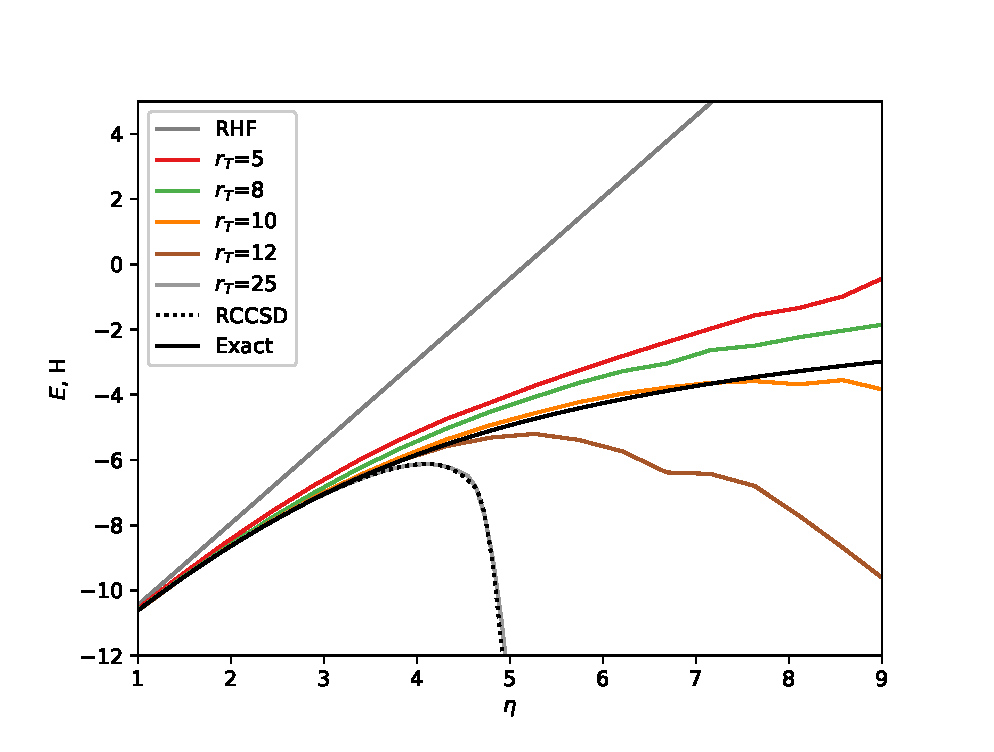
\includegraphics[width=\columnwidth]
{figures/tcc_strong_correlation/energy_vs_u_10_sites_cpd_rccsd}
%\caption{10 sites}
%\label{fig:energy_vs_u_10_sites_cpd_rccsd}
%\end{subfigure}
\caption{Energy behavior for different ranks of CP decomposition of amplitudes. 
Hubbard model at half-filling, 10 sites}
\label{fig:energy_vs_u_cpd}
\end{figure}
%
Figure~\ref{fig:energy_vs_u_cpd} shows the dependence of the total energy 
on the interaction strength $\eta$. As expected, conventional RCCSD provides 
good description of Hubbard rings at low $\eta$, and systematically 
overestimates the energy as the system becomes strong correlated. CPD-RCCSD, 
however, demonstrates a surprising effect. If one chooses the approximation to 
doubles amplitudes to be low 
rank, the incorrect behavior of the original RCCSD method may be fixed. As the 
rank in increased, the solutions of CPD-RCCSD gradually change behavior between 
the one of Hartree-Fock (no correlation) to conventional RCCSD 
(overestimation of correlation energy), as can be seen on 
Figure~\ref{fig:energy_vs_u_cpd}. This situation, however, is not 
specific to CPD-RCCSD, and is also observed with THC-RCCSD (see 
Figure~\ref{fig:energy_vs_u_thc}).
%
\begin{figure}[ht!]
\centering
%\begin{subfigure}{0.75\textwidth}
%\centering
%\includegraphics[width=1\linewidth]
%{figures/tcc_strong_correlation/energy_vs_u_6_sites_thc_rccsd}
%\caption{6 sites}
%\label{fig:energy_vs_u_6_sites_thc_rccsd}
%\end{subfigure}
%\begin{subfigure}{0.75\textwidth}
%\centering
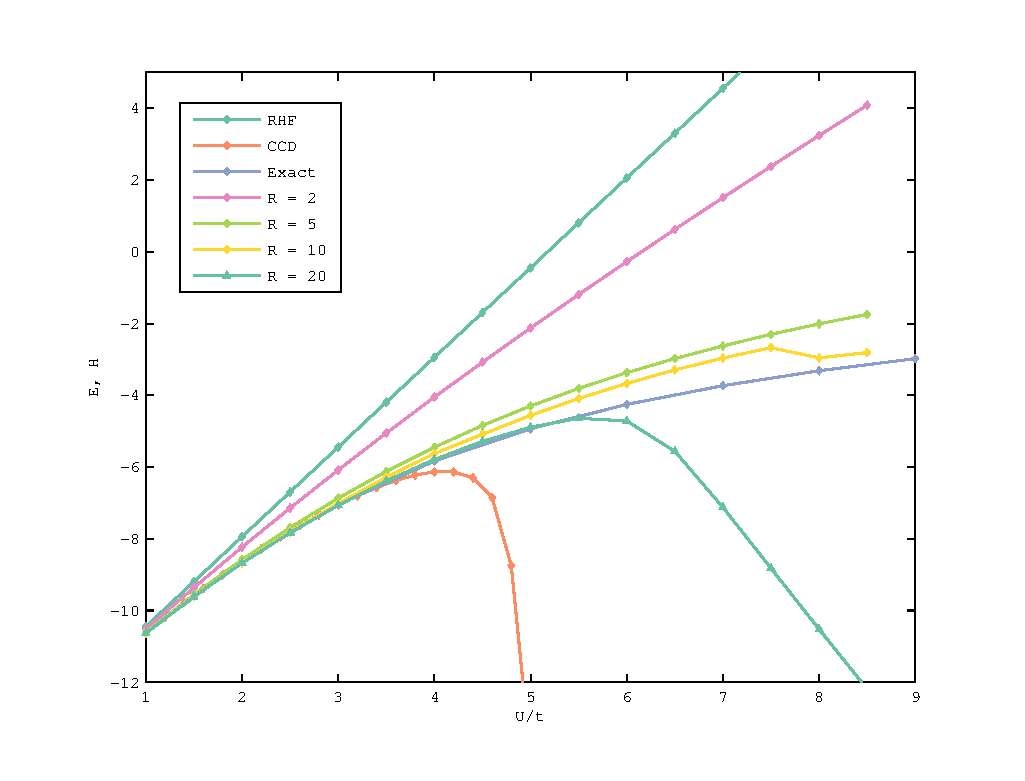
\includegraphics[width=\columnwidth]
{figures/tcc_strong_correlation/energy_vs_u_10_sites_thc_rccsd}
%\caption{10 sites}
%\label{fig:energy_vs_u_10_sites_thc_rccsd}
%\end{subfigure}
\caption{Energy behavior for different ranks of THC decomposition of 
amplitudes. Hubbard model at half-filling, 10 sites}
\label{fig:energy_vs_u_thc}
\end{figure}
%
The difference in case of THC-RCCSD is that the overcorrelation happens at 
slightly larger ranks (compare, for example, $r_{T} = 5$ and $r_{T} = 10$ 
between Figures~\ref{fig:energy_vs_u_cpd} and \ref{fig:energy_vs_u_thc}). Both 
methods, however, reproduce standard RCCSD when sufficiently large ranks of the 
decompositions are chosen, as one may expect.

The results observed with Hubbard Hamiltonian do not change qualitatively in 
case of molecular systems. Figure~\ref{fig:energy_vs_d_cc-pvdz} 
demonstrates the effect of rank restriction in CPD-RCCSD for the calculation of 
the dissociation curve of nitrogen. With rank equal 4 the solution has a 
correct behavior at the dissociation limit, while for larger ranks CPD-RCCSD 
approximates standard RCCSD. The rank restricted solutions, however, miss a 
fair amount of weak correlation energy (e.g. near the equilibrium exact and 
CPD-RCCSD curves are far apart), which plays a major role in molecular systems. 
Having seen the behavior of rank restricted approximate coupled cluster for a 
wide range of systems, we would like to provide an interpretation of the 
observed effect.
%
\begin{figure}[!ht]
\centering
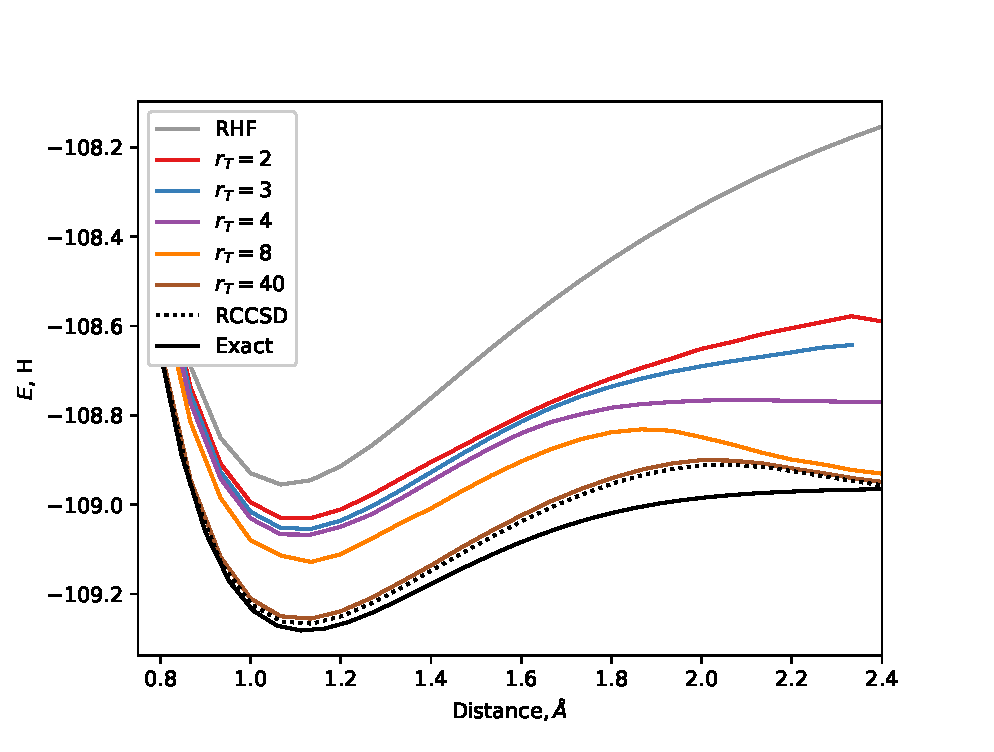
\includegraphics[width=\columnwidth]
{figures/tcc_strong_correlation/energy_vs_d_cc-pvdz}
\caption{Dissociation of nitrogen. CPD-RCCSD energies with different ranks 
$r_{T}$ in amplitude approximation}
\label{fig:energy_vs_d_cc-pvdz}
\end{figure}
%

\subsection{Tentative explanation}
To explain the observed effect one may look at 
different parameters of CPD-RCCSD solutions. In 
Figure~\ref{fig:t2_norms_vs_u_10_sites_cpd_rccsd} the dependence of the norm of 
the 
${}^2T$ amplitudes as a function of rank and on-site repulsion is shown. As the 
graph illustrates, the norm of the doubles amplitudes in the physically 
proper-behaving low rank solutions is lower than the norm of ${}^2T$ amplitudes 
in conventional RCCSD. In contrast, as the ranks grow and CPD-RCCSD starts 
to overcorrelate there is a sharp increase in the amplitude norm to values even 
higher than the standard RCCSD would yield. For example, the solution with 
$r_{T} = 12$, which significantly overcorrelates at $\eta > 6$ (see 
Figure~\ref{fig:energy_vs_u_cpd}, yellow line) also has large 
norm of ${}^2T$ amplitudes starting at the same values of $\eta$ 
(Figure~\ref{fig:t2_norms_vs_u_10_sites_cpd_rccsd}, yellow line). 
The growth of cluster amplitudes was identified as the major problem of the CC 
\emph{ansatz} at strong correlation.\cite{degroote2016polynomial}
%
\begin{figure}[ht]
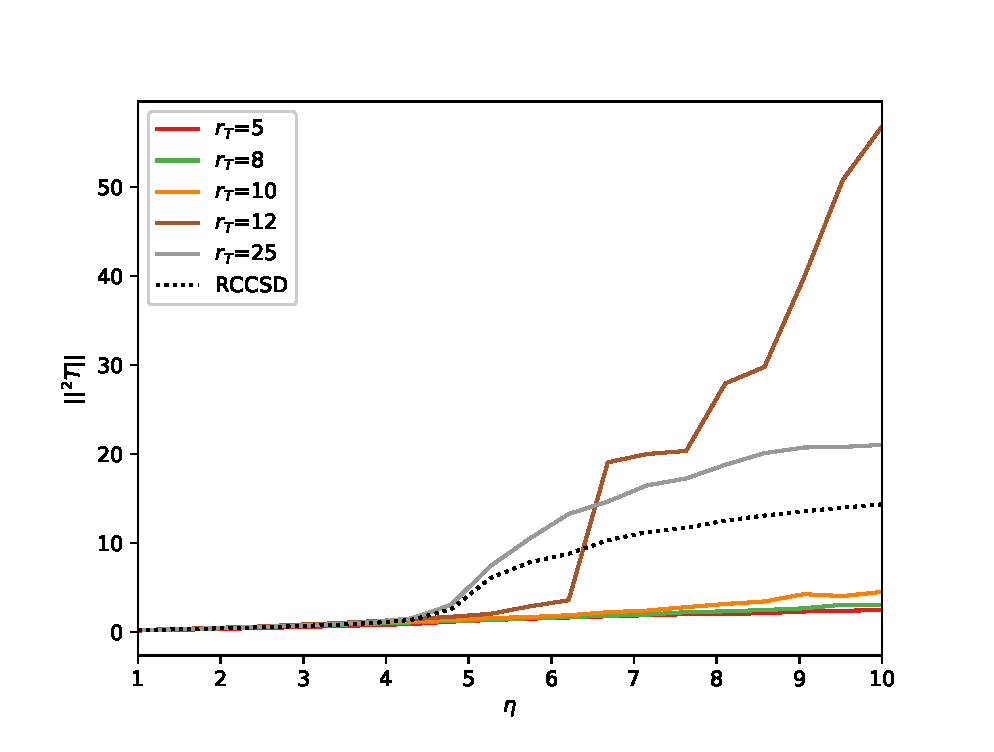
\includegraphics[width=\columnwidth]
{figures/tcc_strong_correlation/t2_norms_vs_u_10_sites_cpd_rccsd}
\caption{Norm of ~ ${}^2T$ amplitudes for different ranks $r_{T}$ in CPD-RCCSD 
calculations. Hubbard model at half-filling, 10 sites.
\label{fig:t2_norms_vs_u_10_sites_cpd_rccsd}}
\end{figure}
%
It was demonstrated by M. Degroote\emph{et al.}~\cite{degroote2016polynomial} 
that in strong correlation regime the magnitude of amplitudes of higher order 
(e.g. triples, quadruples, etc.) in standard restricted CC increases with 
the rank of excitation.

Since CC theory uses an exponential parameterization 
of the wavefunction, e.g. $|\phi \rangle = e^{T} | 0 \rangle$, where $T = {}^1T 
+ {}^2T + {}^3T + \ldots$ (see Chapter~\ref{ch:tcc} for more details), there is 
no natural truncation of the CC excitation operator at strong correlation. 
In a series of works in our group\cite{degroote2016polynomial, 
gomez2017attenuated, qiu2017projected2, hermes2017combining} alternative 
similarity transformations (e.g. non-exponential) were explored, 
which have an excellent accuracy at strong correlation. In those CC-like methods 
the amplitudes do not satisfy the residual equations of standard coupled 
cluster and have smaller norms, which decrease with the order of excitation, due 
to the renormalization of higher order amplitudes. It can be argued that the 
(truncated) exponential \emph{ansatz} of coupled cluster is ill-posed in strong 
correlation setting. By forcing the solution to satisfy CC residual equations 
with excitation operators of low order one makes them significantly deviate from 
the true eigenstates of the Hamiltonian.

It is interesting to note that the low-rank solutions in tensor structured CC 
do not satisfy the CC residual equation either, as 
Figure~\ref{fig:r2_norms_vs_u_10_sites_cpd_rccsd} makes clear. The 
individual factors in the decomposition of amplitudes, however, \emph{do} 
satisfy their own ALS-like equations (see Chapter~\ref{ch:tcc}). The CC 
residuals are large for low-rank solutions and sharply drop as 
CPD-RCCSD amplitudes approach regular RCCSD amplitudes (compare $r_{T} = 8$ 
and $r_{T} = 25$ in 
Figures~\ref{fig:energy_vs_u_thc},~\ref{fig:t2_norms_vs_u_10_sites_cpd_rccsd} 
and~\ref{fig:r2_norms_vs_u_10_sites_cpd_rccsd}). Rank restriction of the 
amplitudes can thus be viewed as a way to regularize conventional CC equations 
in strong correlation regime. We would like to point out that similar 
regularization schemes (called "dropout regularization") are ubiquitous in 
machine learning literature.~\cite{srivastava2014dropout, wan2013regularization} 
The latter rises a question whether other regularization approaches, like 
standard $l_{2}$-norm regularization, can be applied in coupled cluster method.
%
\begin{figure}[ht]
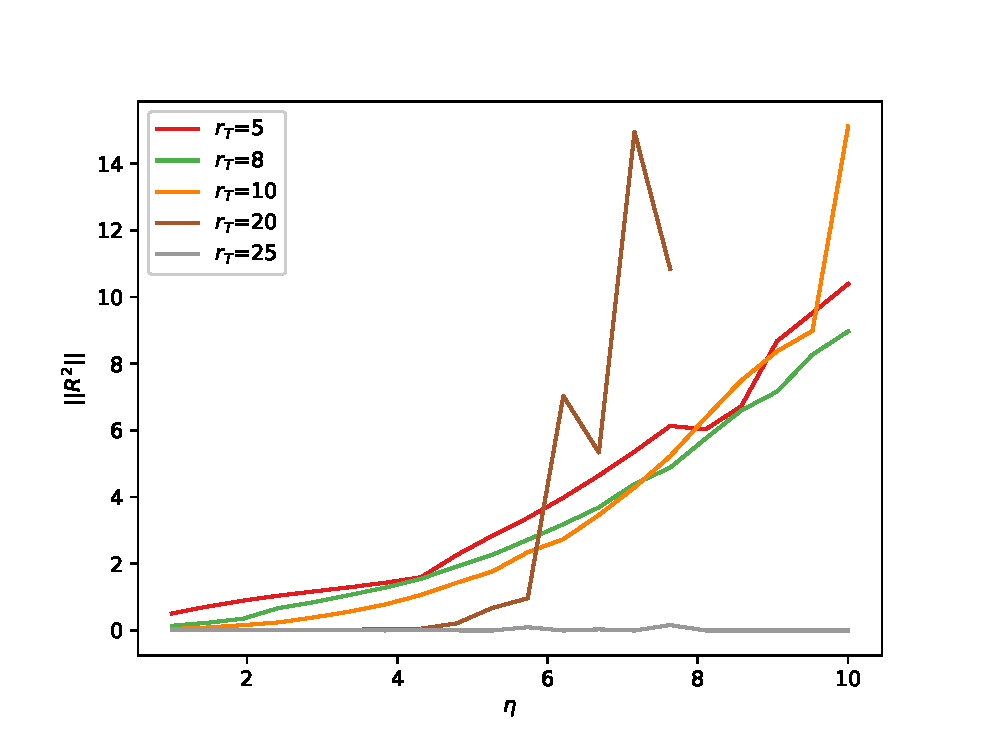
\includegraphics[width=\columnwidth]
{figures/tcc_strong_correlation/r2_norms_vs_u_10_sites_cpd_rccsd}
\caption{Norm of ~${}^2T$ residuals for different ranks $r_{T}$ in CPD-RCCSD 
calculations. Hubbard model at half-filling, 10 sites}
\label{fig:r2_norms_vs_u_10_sites_cpd_rccsd}
\end{figure}
%

\subsection{Conclusions}
The strong correlation regime poses a hard problem for most many-body methods. 
Coupled Cluster methods, while being very effective for weakly correlated 
systems, fail when the strong correlation dominates. Recently a series of 
promising CC-like theories was developed in our 
group.\cite{degroote2016polynomial, gomez2017attenuated, 
qiu2017projected2, hermes2017combining} 
The problem of these theories, however, is that the explicit form of equations 
depends on the symmetry of the Hamiltonian responsible for the onset of strong 
correlation, and the idea is hard to generalize for arbitrary Hamiltonians. On 
the other hand, rank restriction in tensor structured CC provides another way to 
regularize the solutions of standard coupled cluster at strong correlation, 
independently of the form of the Hamiltonian. More research is needed to make 
this approach practically applicable, but we believe the idea may be 
interesting in future method development.